
\section{Architecture Integration}

\subsection{Model Support Matrix}

\begin{table}[H]
\centering
\small
\begin{tabular}{llllll}
\toprule
\textbf{Architecture} & \textbf{Class} & \textbf{Nested?} & \textbf{RoPE?} & \textbf{GQA?} & \textbf{Verified} \\
\midrule
DistilBERT & \texttt{MultiHeadSelfAttention} & No & No & No &  \\
RoBERTa & \texttt{BertSelfAttention} & Yes & No & No & 0.85 \\
GPT-2 & \texttt{GPT2Attention} (Conv1D) & No & No & No & 0.85 \\
Qwen3.5 & \texttt{Qwen3Attention} & No & Yes & Yes & 0.85 \\
\bottomrule
\end{tabular}
\end{table}

\subsection{Weight Transfer}

The \texttt{copy\_weights} method handles three extraction patterns:

\subsubsection{GPT-2 (Fused Conv1D)}

\begin{lstlisting}
if hasattr(src, "c\_attn"):
    c\_w = src.c\_attn.weight.data.clone()
    if src.c\_attn.\_\_class\_\_.\_\_name\_\_ == "Conv1D":
        c\_w = c\_w.t()
    q\_w, k\_w, v\_w = c\_w.chunk(3, dim=0)
\end{lstlisting}

\subsubsection{RoBERTa (Nested)}

We unwrap the nested structure:

\begin{lstlisting}
elif hasattr(src, "self"):
    s = src
    while hasattr(s, "self") and not any(
        hasattr(s, attr) for attr in ["query", "key", "value"]
    ):
        s = s.self
    # Now s is BertSelfAttention with query/key/value
\end{lstlisting}

The output projection is taken from \texttt{src.output.dense}.

\subsubsection{DistilBERT (Flat)}

Direct extraction:

\begin{lstlisting}
extracted["q"] = src.q\_lin.weight.data
extracted["k"] = src.k\_lin.weight.data
extracted["v"] = src.v\_lin.weight.data
extracted["o"] = src.out\_lin.weight.data
\end{lstlisting}

\subsection{Nested Encoder Bypass}

For RoBERTa, we set \texttt{is\_nested\_encoder = True} and skip our own \texttt{out\_proj}:

\begin{lstlisting}
if self.is\_nested\_encoder:
    return context, None
output = self.out\_proj(context)
\end{lstlisting}

The outer \texttt{BertSelfOutput.dense} applies the projection.

\subsection{GQA Support}

For Qwen with $H_{kv} < H$:

\begin{lstlisting}
if self.num\_heads != self.num\_kv\_heads:
    K = repeat\_kv(K, self.num\_heads // self.num\_kv\_heads)
    V = repeat\_kv(V, self.num\_heads // self.num\_kv\_heads)
\end{lstlisting}

This is applied \textbf{before} the joint feature computation.

\subsection{RoPE Support}

Partial RoPE supported via \texttt{apply\_rotary\_pos\_emb}.

\subsection{Injection Algorithm}

\textbf{Algorithm 3:} Inject Routing Attention
\begin{lstlisting}
Input:  layer  , config, old\_attn
Output: new attention module

1: new $\leftarrow$ RoutingAttention(config, pretrained\_attn=old\_attn)
2: if layer.attention.self: 
3:     layer.attention.self $\leftarrow$ new; new.is\_nested\_encoder $\leftarrow$ True
4: elif layer.self\_attn: layer.self\_attn $\leftarrow$ new
5: elif layer.attn: layer.attn $\leftarrow$ new
6: elif layer.self: layer.self $\leftarrow$ new; new.is\_nested\_encoder $\leftarrow$ True
7: return new
\end{lstlisting}

\subsection{Failure Handling}

\begin{table}[H]
\centering
\small
\begin{tabular}{lll}
\toprule
\textbf{Failure} & \textbf{Detection} & \textbf{Response} \\
\midrule
Missing weight & \texttt{copy\_weights} sets \texttt{(None, None)} & Random init \\
Shape mismatch & Runtime check & Truncate to min \\
Zero norm & \texttt{RuntimeError} raised & Injection aborts \\
Injection exception & try/except in \texttt{inject\_routing} & Return \texttt{None} \\
\bottomrule
\end{tabular}
\end{table}

\subsection{`RuntimeError` on Zero Norm}

Unlike other modules, this one \textbf{raises} if a weight has near-zero norm:

\begin{lstlisting}
w\_norm = float(torch.norm(target\_mod.weight.data).item())
if w\_norm \textless{} 1e-4:
    raise RuntimeError(f"RoutingAttention weight verification failed for '{proj\_key}': "
                       f"norm too small ({w\_norm:.2e})")
\end{lstlisting}

\textbf{This is a bug.} If any projection weight is legitimately small, the 
injection fails for the entire model. Consider replacing with a warning.

\subsection{Double-Injection Guard}

The \texttt{inject\_routing} function does \textbf{not} check for prior injection. Running 
it twice could corrupt the model.

\subsection{Diagnostics}

\begin{lstlisting}
# Verify injection
for name, mod in model.named\_modules():
    if 'routing' in type(mod).\_\_name\_\_.lower():
        print(name, type(mod).\_\_name\_\_)
\end{lstlisting}

\subsection{Common Pitfalls}

\subsubsection{Cluster IDs on Padded Sequences}

Padding tokens are included in k-means clustering, which may distort 
centroids. Ideally, exclude padding before clustering.

\subsubsection{Token-0 Anchor on Long Sequences}

If token 0 is itself a padding token (rare), the anchor becomes meaningless. 
Consider using the first valid token instead.

\subsubsection{Nested Encoder Double-Projection}

If \texttt{is\_nested\_encoder} is wrong, the output projection is applied twice.
\begin{lstlisting}

---
\end{lstlisting}

\begin{figure}[H]
\centering
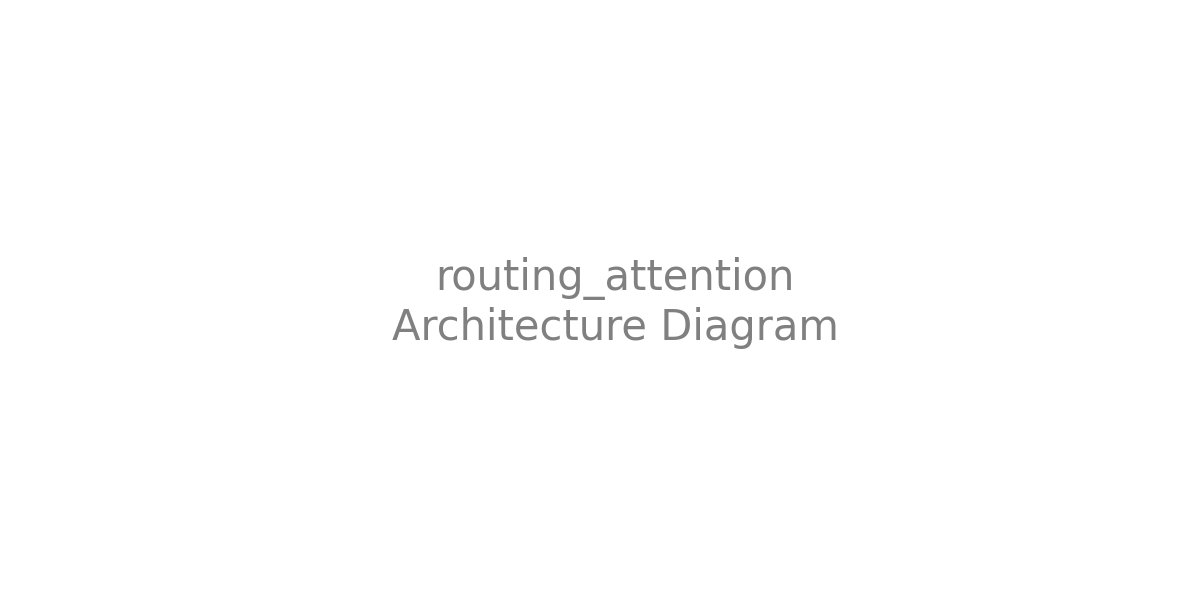
\includegraphics[width=\linewidth]{figures/architecture.png}
\caption{High-level architectural diagram of routing\_attention.}
\label{fig:arch_routing-attention}
\end{figure}

